%PRECEDENTE: funzioni-complesse
\chapter{Le trasformazioni di M\"{o}bius}

Le trasformazioni di M\"{o}bius sono marticolari tipi di funzioni della forma:
\begin{equation}
M(z)=\frac{az+b}{cz+d}
\end{equation}
dove $a,b,c,d\in C$ tali che $ad-cb \neq 0$.
\\A tale trasformazione (definita su $\C$ a valori in $\C$) può essere associata una matrice, composta da:
\[
L_M =
\begin{pmatrix}
a	&b\\
c	&d
\end{pmatrix}
\]                                  
La scrittura tramite matrice è comoda nella composizione di due trasformazioni di M\"{o}bius, perchè possiamo trovare la trasformazione associata sempicemente eseguendo il prodotto fra le due matrici; infatti:
$$M'(M(z))=\frac{a'M(z) + b'}{c'M(z) + d'}=\frac{a'(az+b)+b'(cz+d)}{c'(az+b)+d'(cz+d)}=$$
$$=\frac{(a'a+b'c)z+(a'b+b'd)}{(c'a+d'c)z+(c'b+d'd)}$$
Che è lo stesso risultato che otterremmo eseguendo il prodotto fra matrici $L_{M'M}=L_{M'}L_M$.
\\Allo stesso tempo, possiamo facilmente invertire la trasformazione semplicemente trovando la matrice inversa.
 
La mappa lineare $z'=az+b$ e l'inversione $z'=\frac{1}{z}$ sono particolari tipi di trasformazioni di M\"{o}bius con matrice associata:
\[
L_{lineare} =
\begin{pmatrix}
a	&b\\
0	&1
\end{pmatrix}
\]
\[
L_{inversione} =
\begin{pmatrix}
0	&1\\
1	&0
\end{pmatrix}
\]
Possiamo scrivere ogni trasformazione di M\"{o}bius come composizione di mappe lineari e inversioni; infatti, abbiamo che:
\[
\begin{pmatrix}a&b\\c&d\end{pmatrix} = \begin{pmatrix}-\frac{ad-bc}{c}&\frac{a}{c}\\0&1\end{pmatrix}\begin{pmatrix}0&1\\1&0\end{pmatrix}\begin{pmatrix}c&d\\0&1\end{pmatrix}
\]
Dato che sia l'inversione sia la mappa lineare mandano cerchi in cerchi, si ha che ogni mappa di M\"{o}bius conserva tale proprietà.

Per determinare la mappa in questione, basta semplicemente prendere tre punti nel piano di partenza e fissarne le immagini; in questo modo, possiamo fissare univocamente la mappa che unisce i due piani.

Introduciamo ora la Sfera di Riemann, cioè una sfera tangente al piano complesso nell'origine degli assi; dal ''polo nord'', cioè dal punto diametralmente opposto rispetto al punto di  tangenza della sfera, possiamo raggiungere ogni punto del piano attraverso un segmento che intersecherà una e una sola volta la sfera (a parte l'estremo vincolato al polo). In questo modo, abbiamo una corrispondenza biunivoca fra i punti nel piano e i punti sulla sfera.\\
Grazie a questa mappa, possiamo trasferire tutte le operazioni dal piano complesso alla superficie della sfera; ad esempio, la distanza fra due punti viene trasferita sulla sfera come la distanza cordale, cioè:
$$|A'-B'|:=d_{cordale}(A,B) \in [0;2r]$$

\begin{figure}[h!]
  \centering
    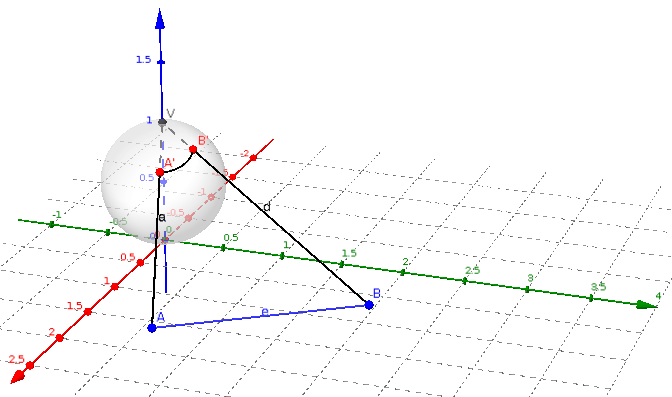
\includegraphics[width=0.5\textwidth]{immagini/sferariemann.png}
\end{figure}

Le trasformazioni di M\"{o}bius che conservano la distanza cordale tra due punti e hanno $ad-bc=1$ corrispondono a matrici $2 \times 2$ in $SU(2)$, cioè lo spazio delle matrici $2 \times 2$ unitarie.

%SUCCESSIVO: completezza-C